%! Author = danielmendes
%! Date = 29.11.24

\chapter{Optimierungen von Datentypen}\label{ch:data-types}

Das erste Thema, das wir in Bezug auf die Performance - Optimierung von Datenbanken betrachten, sind die unterschiedlichen Datentypen und ihre Effizienzsteigerungen.
Bei der Auswahl des korrekten Datentyps gibt es unterschiedliche Faktoren, die vom jeweiligen Typen abhängen.
Es gibt aber auch allgemeinere Prinzipien, die auf fast alle Datentypen angewendet werden können.

\section{Allgemeine Faktoren}\label{sec:data-types-allgemeine-faktoren}

Bei der Erstellung von Tabellen sollte man folgende Schritte für die Auswahl von Datentypen befolgen (\cite[pp. 115--145]{schwartz2012high}).
Zunächst muss die allgemeine Klasse der Typen, wie beispielsweise numerisch, Zeichenketten oder zeitbezogen, festgelegt werden.
Anschließend sollte der spezifische Typ ausgewählt werden.
Für numerische Daten kommen beispielsweise Ganzzahlen wie \texttt{INT} oder Fließkommazahlen wie \texttt{FLOAT} und \texttt{DOUBLE} infrage.
Die spezifischen Typen können dieselbe Art von Daten speichern, unterscheiden sich jedoch im Bereich der Werte, die sie speichern können.
Auch sind sie unterschiedlich in der Precision (Genauigkeit), die sie erlauben und dem physischen Speicherplatz, den sie entweder auf der Festplatte oder im Arbeitsspeicher benötigen.
Einige Datentypen haben auch spezielle Verhaltensweisen und Eigenschaften.

Allgemein gilt für Datentypen, dass kleiner besser ist, weshalb man den kleinstmöglichen Datentypen wählen sollte, den man speichern kann und der die vorhandenen Daten entsprechend repräsentieren kann.
Dadurch wird zum einen weniger Speicherplatz (In-Memory und CPU-Cache) in Anspruch genommen, was meistens zu schnelleren Abfragen führt.
Zum anderen spricht für die Benutzung von kleinstmöglichen Typen die einfache Typveränderung.
Wenn die vorhandenen Daten falsch eingeschätzt wurden und nachträglich ein größerer Datentyp benötigt wird, kann der Typ ohne größere Probleme vergrößert werden.
Eine weitere allgemeine Richtlinie ist die Einfachheit von Datentypen.
Damit ist beispielsweise gemeint, dass Integer einfach zu verarbeiten ist als Character, weshalb man immer einen Integer wählen sollte, wenn man durch ihn die Daten korrekt abbilden kann.
Dies liegt daran, dass weniger CPU-Zyklen benötigt werden, um Operationen auf einfacheren Datentypen zu verarbeiten.
Bei dem Beispiel mit Integer und Character liegt dies an den Character Sets und Sortierregeln, die den Character-Vergleich erschweren.

Die letzte allgemeine Regel, die Performancegewinne bringt, ist die Vermeidung von \texttt{NULL}.
Viele Tabellen enthalten NULLABLE Spalten, selbst wenn die Anwendung kein NULL (Fehlen eines Wertes) speichern muss, da dies die Standardeinstellung ist.
Daher ist es am besten solche Spalten bei der Tabellenerstellung mit dem Identifier \texttt{NOT NULL} zu definieren.
Wenn allerdings \texttt{NULL}-Werte gespeichert werden sollen, dann sollte der Identifier nicht genutzt werden.
Für MySQL ist es dann schwieriger Abfragen zu optimieren, da dadurch Indizes, Indexstatistiken und Wertevergleiche mehr Speicherplatz benötigen und komplizierter werden.
Dies liegt daran, dass indizierte nullable Spalten ein zusätzliches Byte pro Eintrag gebrauchen, was dazu führen kann, dass ein Index mit fester Größe in einen variablen Index umgewandelt wird.
Allerdings fällt die Leistungssteigerung, die durch die Änderung von \texttt{NULL}-Spalten in \texttt{NOT NULL} erzielt wird, in der Regel gering aus.
Besonders bei Verwendung von Indizes sollte aber darauf geachtet werden.

MySQL unterstützt auch viele Aliase, z.B. \texttt{INTEGER}, \texttt{BOOL}, \texttt{NUMERIC}.
Diese Aliase können verwirrend sein, aber sie beeinflussen nicht die Performance.
Wenn eine Tabelle mit einem aliasierten Datentyp erstellt wird und die Tabelle mit SHOW CREATE TABLE untersucht wird, fällt auf, dass statt des aliasierten Datentyps der Basistyp angezeigt wird, da der aliasierte Datentyp intern in den Basistyp umgewandelt wurde.

\section{Einzelne Datentypen und weitere Faktoren}\label{sec:data-types-einzelne-datentypen-und-weitere-faktoren}
Bevor wir untersuchen, ob die eben beschriebene Prinzipien tatsächlich einen Einfluss auf die Performance haben, müssen die speziellen Verhaltensweisen der bekanntesten Datentypen betrachtet werden.

Für nummerische Datentypen gibt es die Wahl zwischen Ganzzahlen und Fließkommazahlen.
Die spezifischen Typen unterscheiden sich nur in der Anzahl der Bits, die sie speichern können.
\texttt{SMALLINT} kann 16 Bits speichern, während \texttt{INT} 32 und \texttt{BIGINT} 64 Bits speichern kann.
Dementsprechend verändert sich auch der mögliche Wertebereich der Zahlen, die durch den Speicherplatz abgedeckt sind.
Mit den optionalen \texttt{UNSIGNED} - Attribute können keine negativen Werte gespeichert werden können, dafür verdoppelt sich aber die obere Grenze der Positiven.
Zeitgleich bleiben der Speicherplatz und die Leistung gleich.
Die Berechnung der Wertebereiche für den default, bzw.\ mit dem Signed-Attribut, erfolgt in~\ref{eq:equation-signed} und mit dem Unsigned - Attribut in~\ref{eq:equation-unsigned}.

\vspace{-4mm}
\begin{gather}
    \text{Signed: } -2^{(N-1)} \text{ bis } 2^{(N-1)} - 1\label{eq:equation-signed} \\
    \text{Unsigned: } 0 \text{ bis } 2^N - 1\label{eq:equation-unsigned}
\end{gather}

\textbf{Hinweis:} $N$ entspricht der Anzahl der Bits.
\vspace{4pt}

Beispiel für 8 Bits:
\begin{itemize}
    \item \text{SIGNED:} -128 \text{ bis } 127
    \item \text{UNSIGNED:} 0 \text{ bis } 255
\end{itemize}

Eine Breitenangabe wie \texttt{INT(11)} beeinflusst nur die Anzeige und nicht den Wertebereich oder die Speicheranforderungen.
Um dies zu beweisen, können wir die folgende Table erstellen.

\lstinputlisting[
    language=sql,
    caption=SQL-Befehl zur Erstellung der Testtabelle,
    label={lst:testint_create_sql},
    style=custom_daniel,
]{Scripts/Data_Types/01_testint_create.sql}

Da wir den für die beiden Variablen den Typen INT gewählt haben und wir überprüfen wollen, ob die Breitenangabe einen Einfluss auf die Speicheranforderungen hat, können wir die Grenzen des Wertebereichs für INT einfügen: -2147483648 und 2147483647.
\lstinputlisting[
    language=sql,
    caption=Inserts und Selects für Testtabelle aus \ref{lst:testint_create_sql},
    label={lst:testint_queries_sql},
    style=custom_daniel,
]{Scripts/Data_Types/02_testint_queries.sql}

\begin{table}[h!]
    \centering
    \caption{Ergebnis der SQL-Abfrage aus \ref{lst:testint_queries_sql}}
    \begin{tabular}{|c|c|}
        \hline
        \textbf{int\_5} & \textbf{int\_11} \\ \hline
        2147483647 & 2147483647 \\ \hline
        -2147483648 & -2147483648 \\ \hline
    \end{tabular}
    \label{tab:int_values}
\end{table}
Für den maximalen Wert von INT werden 32 Bits benötigt: $2^{(32-1)} - 1 = 2147483647$.
\texttt{INT(5)} und \texttt{INT(11)} können beide die Grenzwerte von INT speichern, weshalb wir bestätigt haben, dass die Breitenangabe keinen Einfluss auf die Speicheranforderungen hat, ansonsten hätten wir einen Fehler bei der Einfügung der Werte bekommen.

Ein spezifischer Typ für eine Festkommazahl ist \texttt{DECIMAL}, die auch für die Speicherung von Ganzzahlen geeignet ist.
Außerdem kann man bei einer Festkommazahl auch die Genauigkeit angeben, da die maximale Anzahl der Ziffern vor und nach dem Dezimalpunkt definiert werden.
\texttt{DECIMAL(18, 9)} beispielsweise speichert neun Ziffern vor und nach dem Dezimalpunkt und benötigt dafür 9 Bytes Speicherplatz.
\texttt{DECIMAL} speichert Zahlen in einer binären Zeichenkette (binary string) mit neun Ziffern pro vier Bytes und unterstützt bis zu 65 Ziffern insgesamt.

Zu den Fließkommazahlen gehören die \texttt{FLOAT}- und \texttt{DOUBLE}-Typen, die die standardmäßige Gleitkomma-Arithmetik verwenden und für ungefähre Berechnungen optimiert sind.
\texttt{FLOAT} benötigt 4 Bytes, während \texttt{DOUBLE} 8 Bytes Speicherplatz beansprucht und eine höhere Präzision sowie einen größeren Wertebereich bietet.
Die Gleitkomma-Arithmetik ist aufgrund der nativen Verarbeitung durch die CPU deutlich schneller als die präzise Berechnung mit \texttt{DECIMAL}, bringt jedoch einen gewissen Präzisionsverlust mit sich.
Alternativ kann auch \texttt{BIGINT} genutzt werden, um sowohl die Ungenauigkeit von Gleitkomma-Speicherungen als auch die höheren Kosten der \texttt{DECIMAL}-Arithmetik zu vermeiden.

Die beiden Haupttypen für Zeichenketten sind \texttt{VARCHAR} und \texttt{CHAR}. \texttt{VARCHAR} speichert die Zeichenfolgen mit variabler Länge und benötigt daher weniger Speicherplatz als Typen mit fester Länge, da nur so viel Platz verwendet wird, wie tatsächlich benötigt wird.
Zusätzlich werden ein oder zwei Bytes für die Speicherung der Länge der Zeichenfolge verwendet (1 Byte für < 255 Bytes Zeichenfolge).
Durch diese effiziente Speichernutzung ist VARCHAR der am häufigsten verwendete Datentyp für Zeichenketten, aber es hat auch Nachteile, da Aktualisierungen an den Werten zu wachsenden Zeilen und damit auch zusätzliche Verarbeitung der Speicher - Engine erfordern kann.
Und obwohl die Speicherung von \texttt{hello} in \texttt{VARCHAR(5)} oder \texttt{VARCHAR(200)} gleich viel Speicherplatz benötigt, kann es trotzdem ineffizienter für Sortierungen oder Operationen auf temporären Tabellen sein.
Deshalb sollte trotzdem immer so viel Platz reserviert werden, wie tatsächlich benötigt wird.

\texttt{CHAR} hingegen hat eine feste Länge und MySQL reserviert immer auch den nicht gebrauchten Platz für die angegebene Anzahl an Zeichen.
Daher ist \texttt{CHAR} ideal für sehr kurze Strings oder Werte, die alle nahezu gleich lang sind, da \texttt{VARCHAR(1)} zwei Bytes aufgrund des Längen - Bytes benötigt, \texttt{CHAR(1)} hingegen auch.
Außerdem ändert sich bei CHAR die Speicherstruktur bei Aktualisierungen nicht, weshalb dieser Datentyp besser geeignet ist, wenn die Daten häufig verändert werden.
Hingegen \texttt{VARCHAR} eignet sich besonders, wenn die maximale Länge einer Spalte deutlich größer ist als die durchschnittliche Länge der gespeicherten Werte.

\texttt{DATETIME} und \texttt{TIMESTAMP} können dieselbe Art von Daten speichern und beide haben dabei eine Genauigkeit von einer Sekunde.
\texttt{TIMESTAMP} benötigt aber nur halb so viel Speicherplatz, ist zeitzonenbewusst und verfügt über spezielle Auto-Update-Funktionen.
Allerdings hat \texttt{TIMESTAMP} einen viel kleineren Bereich an erlaubten Werten und manchmal können seine speziellen Fähigkeiten ein Nachteil sein.

\section{Analyse der Benchmarks}\label{sec:data-types-analyse-der-benchmarks}

Der erste Leitsatz, den wir untersuchen, besagt, dass Spalten nach Möglichkeit als \texttt{NOT NULL} deklariert werden sollten.
Für den Nachweis benutzen wir erneut die Kundentabelle (\ref{lst:create_table_kunde}).
Diesmal erstellen wir eine Tabelle, bei der das Attribut \texttt{NOT NULL} für alle Spalten deklariert wird, sowie eine Tabelle ohne dieses Attribut.
Wenn das Attribut nicht deklariert wird, dann können u.a.\ auch \texttt{NULL}-Werte in die Tabelle eingefügt werden.

\vspace{-15pt}
\begin{figure}[H]
    \centering
    \begin{subfigure}[t]{0.48\textwidth}
        \centering
        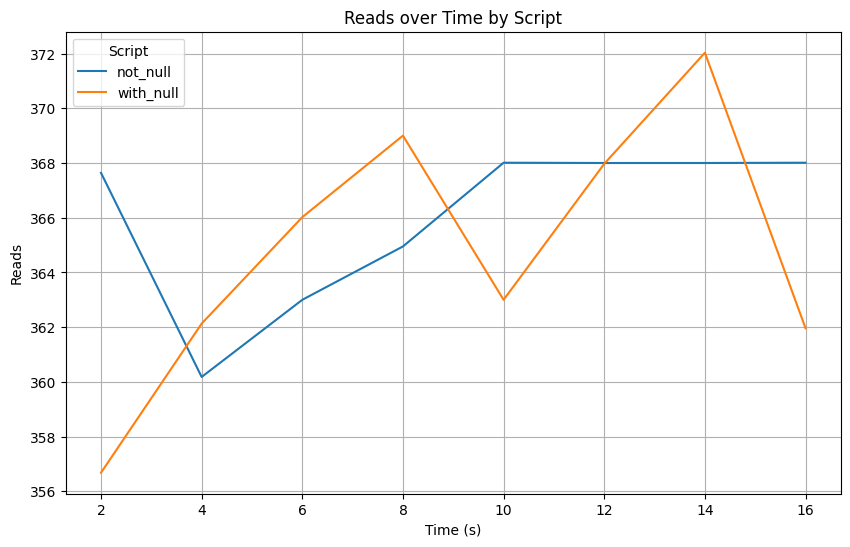
\includegraphics[width=\textwidth]{PNGs/Script/Data_Types/Null/null-check/Reads}
        \caption{Readsabfragen für jeweils 2 Selects}
        \label{data-types-null-reads}
    \end{subfigure}
    \hfill
    \begin{subfigure}[t]{0.48\textwidth}
        \centering
        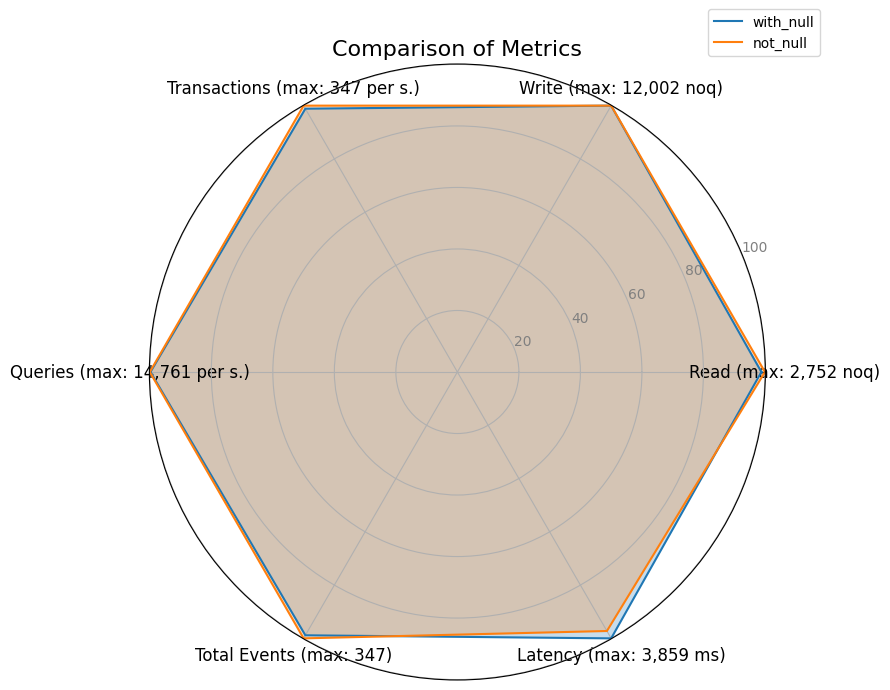
\includegraphics[width=\textwidth]{PNGs/Script/Data_Types/Null/null-check/statistics}
        \caption{Metriken über den kompletten Zeitraum}
        \label{fig:data-types-null-statistics}
    \end{subfigure}
    \caption[Datentypen: Null und Not Null]{Vergleich von Null und Not Null}
\end{figure}
\vspace{-20pt}

In der erstellten Grafik (siehe Abbildung~\ref{data-types-null-reads}) sind die beiden Resultate der Select-Befehle zu sehen, die sowohl einfache WHERE-Klauseln als auch Count- und Group-By-Befehle enthalten.
Anhand der Grafik lässt sich erkennen, dass die Werte für \texttt{NOT NULL} höher liegen als für \texttt{NULL}, bzw \texttt{WITH NULL}.
Höhere Werte bedeuten, dass mehr Abfragen pro Sekunde durchgeführt werden können, was auf eine bessere Performance hindeutet.
Deshalb lässt es sich sagen, dass \texttt{NOT NULL} besser performt als \texttt{NULL}, aber wenn man auf die y-Achse schaut, fällt auf, dass die Werte nicht so weit auseinanderliegen, sondern der Unterschied nur marginal ist.
Daher sollten die Entscheidungen beim Datenbankentwurf nicht hauptsächlich aus Performancegründen getroffen werden, sondern vor allem aus Gründen der Datenintegrität und -konsistenz.

Um zu zeigen, dass man bei der Wahl zwischen unterschiedlichen Datentypen, den simpleren wählen sollte, haben wir erneut die Kundentabelle (\ref{lst:create_table_kunde}) benutzt.
Für diesen Vergleich verändern wir jeweils den Datentyp des Schlüsselattributs der Tabelle.
Zuerst erstellen wir eine Kundentabelle mit einem \texttt{INT}-Primärschlüssel, danach eine mit \texttt{CHAR}.
An den Ergebnissen im Hexagon~\ref{fig:data-types-simpler-statistics} fällt auf, dass die Schreibbefehle in beiden Fällen etwa gleich schnell sind.
Aber bei den Abfragen gibt es deutliche Unterschiede.
Wenn man einen Wertebereich abfragt, dann ist \texttt{INT} deutlich schneller (~50\%) ist als \texttt{CHAR}.
Bei der Sortierung hat \texttt{INT} ebenfalls einen Vorteil gegenüber \texttt{CHAR}, jedoch fallen die Abstände deutlich geringer aus (\ref{data-types-simpler-reads}).

\vspace{-15pt}
\begin{figure}[H]
    \centering
    \begin{subfigure}[t]{0.48\textwidth}
        \centering
        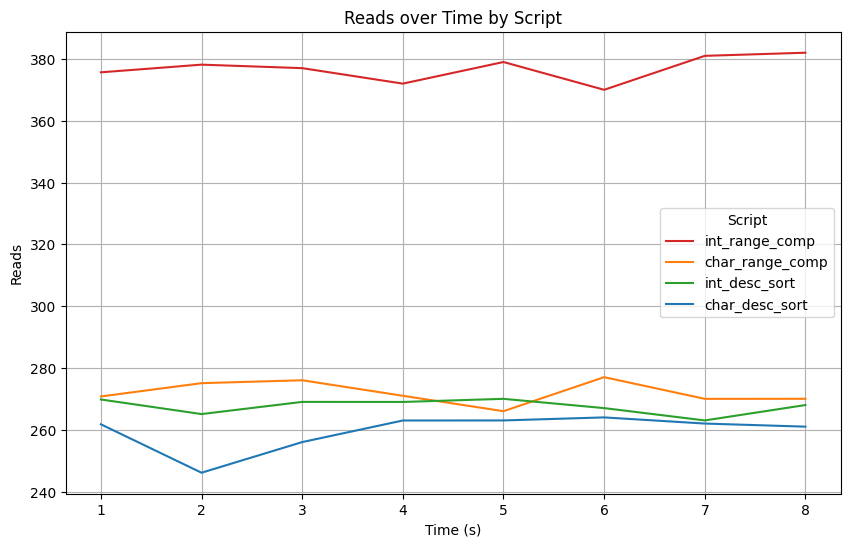
\includegraphics[width=\textwidth]{PNGs/Script/Data_Types/Simpler/int-char/Reads}
        \caption{Vergleich für jeweils 2 unters. Abfragen}
        \label{data-types-simpler-reads}
    \end{subfigure}
    \hfill
    \begin{subfigure}[t]{0.48\textwidth}
        \centering
        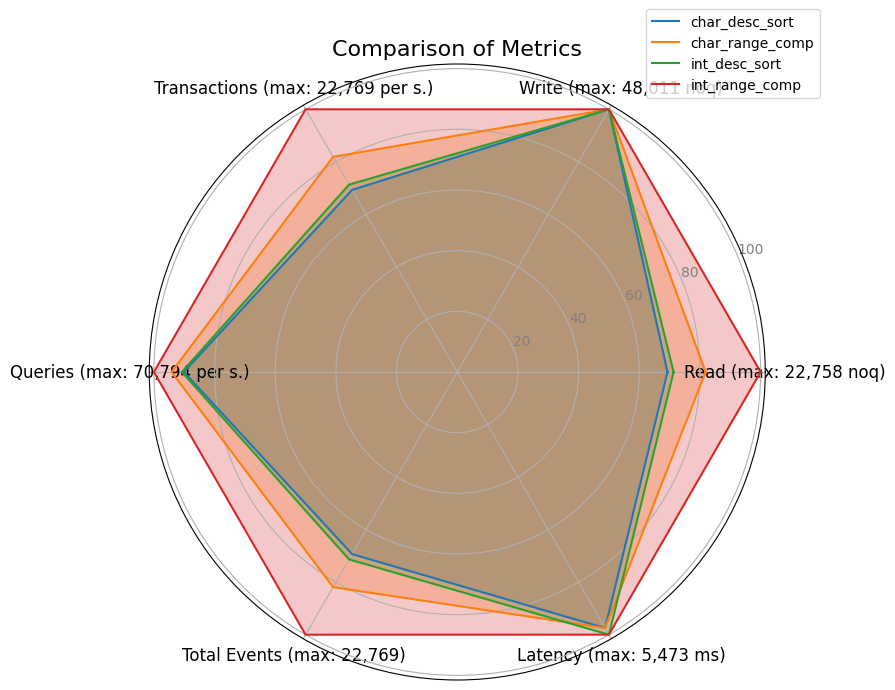
\includegraphics[width=\textwidth]{PNGs/Script/Data_Types/Simpler/int-char/statistics}
        \caption{Kennzahlen über den gesamten Zeitraum}
        \label{fig:data-types-simpler-statistics}
    \end{subfigure}
    \caption[Datentypen: Int und Char]{Vergleich von Int und Char}
\end{figure}
\vspace{-20pt}

Als Letztes wollten wir unterschiedliche Datentypen vergleichen.
Dazu verwenden wir die gleiche Tabelle wie beim Vergleich von \texttt{INT} und \texttt{CHAR}, setzen diesmal jedoch unterschiedliche numerische oder zeichenkettenbasierte Typen als Primärschlüssel ein.
Beim Vergleich der numerischen Typen zeigt sich, dass \texttt{DECIMAL} mit deutlichem Abstand am langsamsten ist (Abbildung~\ref{data-types-smaller-number-type-reads}).
Danach folgt, wie vermutet, der nächstgrößere Datentyp \texttt{BIGINT}.
Auffällig ist, dass der Unterschied zwischen \texttt{INT}, \texttt{MEDIUMINT} und \texttt{SMALLINT} kleiner ist als erwartet.
Dies wird vermutlich aber daran liegen, dass wir die Abfragen nur auf eine Tabelle mit wenigen tausend Datensätzen ausgeführt haben.
In der Praxis mit Hunderttausenden oder Millionen von Datensätzen ist anzunehmen, dass die Unterschiede zwischen den Typen größer wären als in unserem Vergleich.

Beim Vergleich zwischen den beiden Zeichenketten-Typen \texttt{CHAR} und \texttt{VARCHAR} ist unabhängig von der Länge zu erkennen, dass \texttt{VARCHAR} effizienter ist als \texttt{CHAR} (\ref{fig:data-types-smaller-string-type-reads}).
Im ersten Vergleich wurde jeweils eine Länge von 4 Stellen verwendet und beim zweiten Vergleich eine Länge von 64 Stellen.
Bei beiden untersuchten Längen ist \texttt{VARCHAR} schneller als \texttt{CHAR}.
Wenn man sich jedoch die Performance beim Einfügen von Werten anschaut, fällt auf, dass die Unterschiede eher gering sind und es gibt auch stärkere Schwankungen bei den Werten (siehe Abbildung~\ref{fig:data-types-smaller-string-type-writes}).

\vspace{-12pt}
\begin{figure}[H]
    \centering
    \begin{subfigure}[t]{0.48\textwidth}
        \centering
        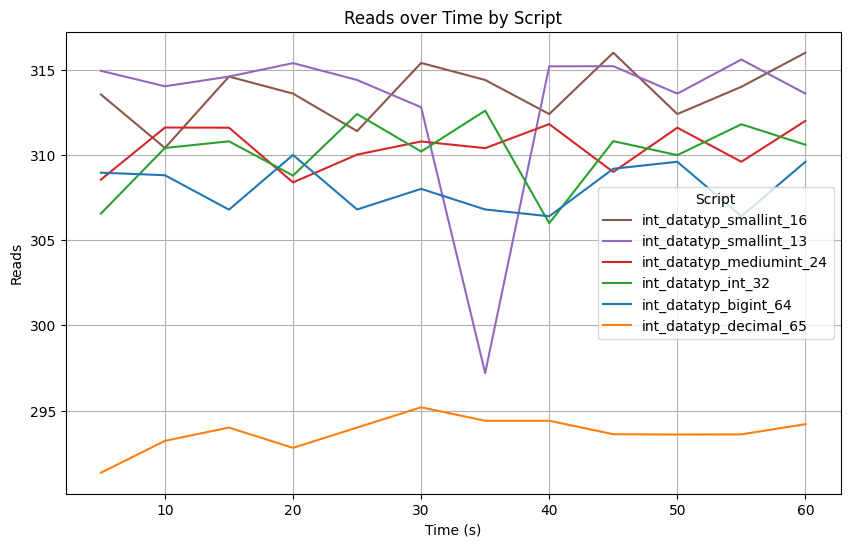
\includegraphics[width=\textwidth]{PNGs/Script/Data_Types/Smaller/number-type/Reads}
        \caption{Unterschiedliche numerische Typen}
        \label{data-types-smaller-number-type-reads}
    \end{subfigure}
    \hfill
    \begin{subfigure}[t]{0.48\textwidth}
        \centering
        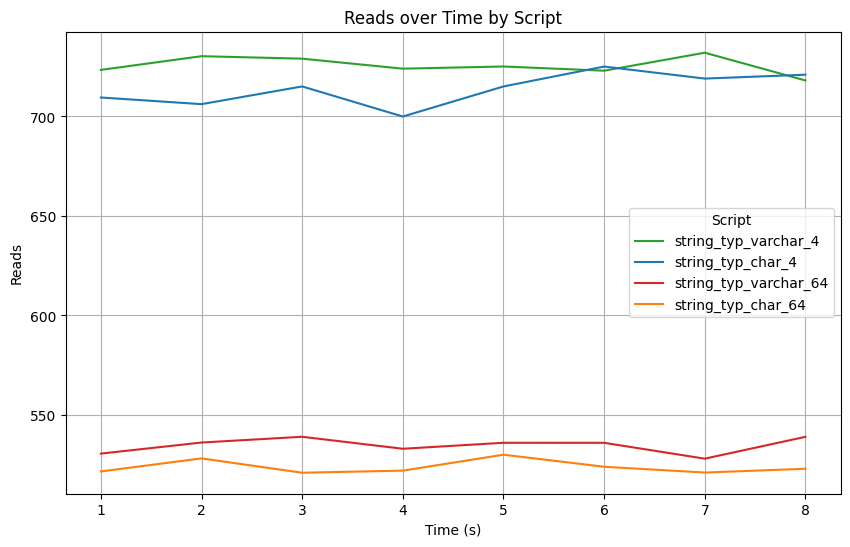
\includegraphics[width=\textwidth]{PNGs/Script/Data_Types/Smaller/string-type/Reads}
        \caption{Unterschiedliche Zeichenketten-Typen}
        \label{fig:data-types-smaller-string-type-reads}
    \end{subfigure}
    \newline
    \begin{subfigure}[t]{0.48\textwidth}
        \centering
        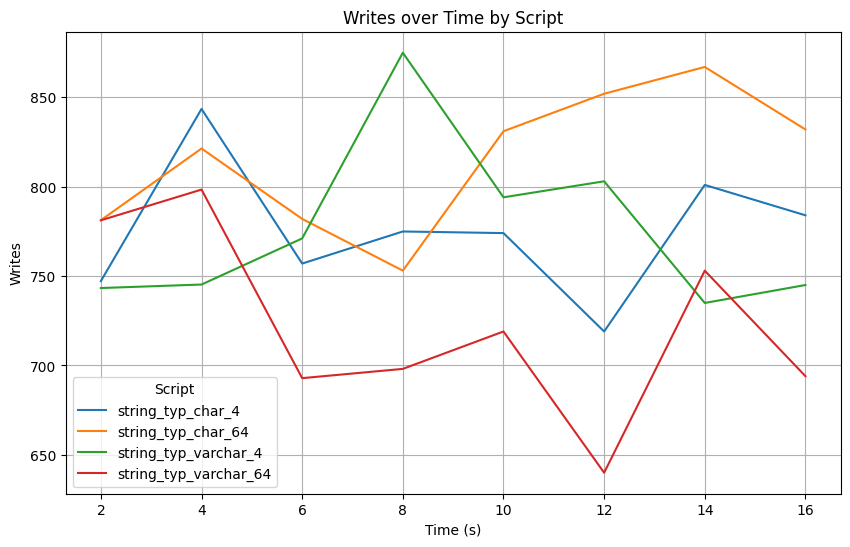
\includegraphics[width=\textwidth]{PNGs/Script/Data_Types/Smaller/string-type/Writes}
        \caption{Bei gleicher Länge der Zeichen}
        \label{fig:data-types-smaller-string-type-writes}
    \end{subfigure}
    \hfill
    \begin{subfigure}[t]{0.48\textwidth}
        \centering
        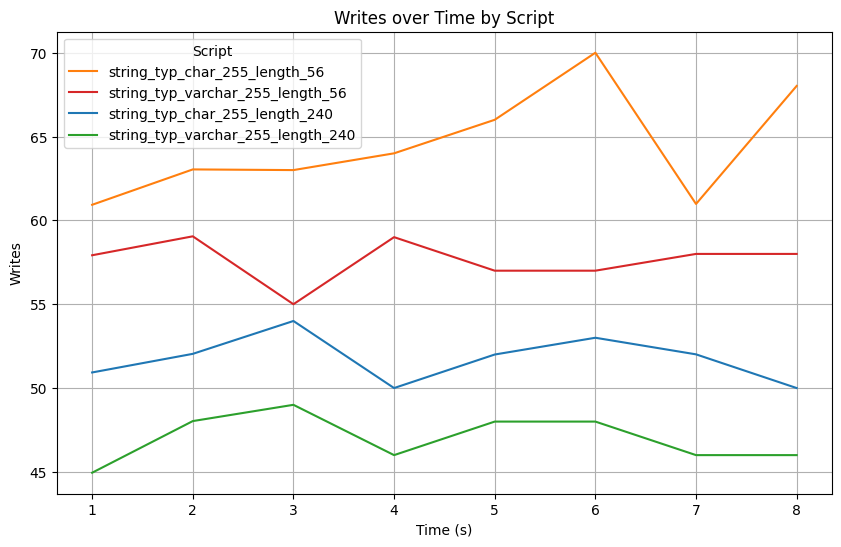
\includegraphics[width=\textwidth]{PNGs/Script/Data_Types/Smaller/string-type-length/Writes}
        \caption{Bei unterschiedlichem Befüllungsgrad}
        \label{fig:data-types-smaller-string-type-length-writes}
    \end{subfigure}
    \caption[Datentypen: Numerische und zeichenkettenbasierte Typen]{Vergleich von unters. numerischen und zeichenkettenbasierten Typen}
\end{figure}
\vspace{-20pt}

Als letzten Vergleich haben beide Zeichenketten-Typen mit der Länge von 255 Stellen definiert, aber dafür mit unterschiedlich vielen Stellen befüllt.
Anschließend haben wir bei beiden Tabellen die Werte aktualisiert und wenige Stellen bei der Namen-Spalte zufällig hinzugefügt.
Wenn man dies tut, dann fällt auf, dass \texttt{CHAR} schneller ist als \texttt{VARCHAR} (\ref{fig:data-types-smaller-string-type-length-writes}).
Zusätzlich wird der Unterschied zwischen den beiden Typen größer, je mehr Stellen befüllt werden.
Damit haben wir gezeigt, dass die Vorteile von \texttt{CHAR} insbesondere bei der Aktualisierung von Werten liegen, während \texttt{VARCHAR} bei der Selektion von Werten besser abschneidet.
Der Grund hierfür ist, dass \texttt{CHAR} die verbleibenden Stellen mit Leerzeichen auffüllt, was zu einem höheren Speicherbedarf führt.